
The BBs for the poly(propyleneimine) (PPI) dendrimer are shown in Figure \ref{fig:PPIBB}.
The core is a diamino butane, intermediary monomer is defined as a tertiary amine in addition to to a secondary amine which is the anchoring point for the core or previous intermediary shell bonding and the terminal is simply a primary amine.
It is important to note that PPI dendrimers are commonly defined differently.
For instance, this tutorial may be adapted to generate a common used PPI dendrimer by removing the secondary amine from the intermediary monomer and modifying the \texttt{[ branches ]} field in \texttt{inter\_PPI.itp}.

\begin{figure}
    \centering
    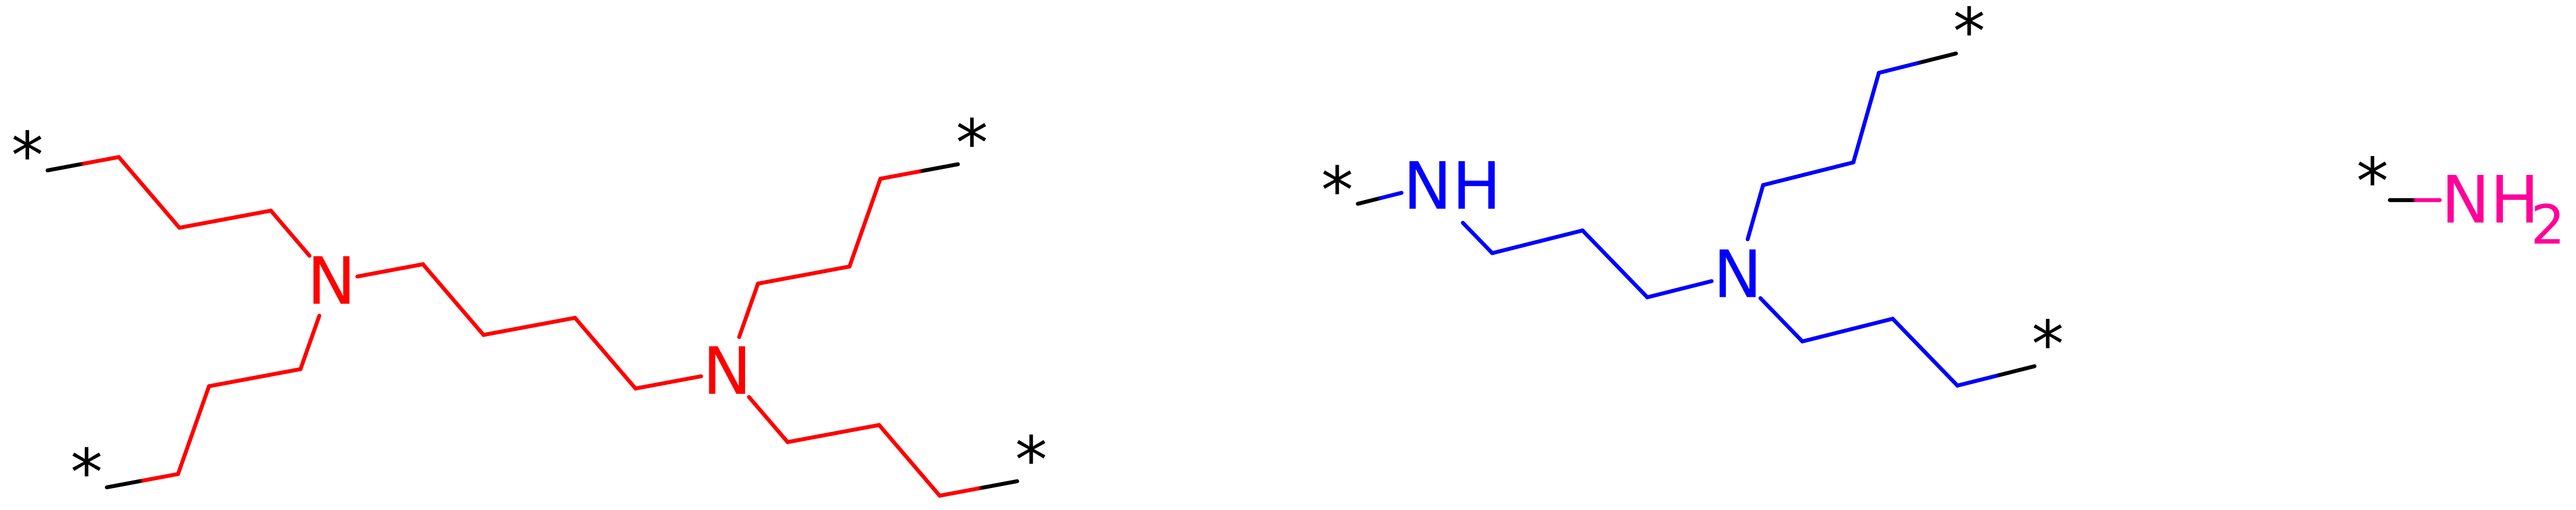
\includegraphics[width=\textwidth]{PPI/PPIBBs.png}
    \caption{PPI dendrimer BBs.
             The core diamine butane block is illustrated in red, the intermediary tertiary amine in blue and the terminal primary amine block is displayed in pink.}
    \label{fig:PPIBB}
\end{figure}

All PPI BBs, in addition to its protonated versions, are provided in the demo directory in pypolybuilder root, which structure is illustrated below:
\begin{lstlisting}
<path/to/pypolybuilder>/demo/gromacs_format/dendrimer/PPI
\end{lstlisting}
\dirtree{%
.1 PPI.
.2 core\_PPI.itp.
.2 inter\_PPI.itp.
.2 ter\_PPI.itp.
.2 list\_param.itp.
.2 run.
.3 PPI.sh.
.3 PPI.top.
.3 mdp.
}

The core\_PPI.itp, inter\_PPI.itp and ter\_PPI.itp files are the MTF for the core, the intermediary and the terminal blocks, respectively.
Once the BBs and the parameters list are successfully built, one can easily run pyPolyBuilder by using the code line (also available in \texttt{how\_to\_run\_this\_example.txt} in demo directory) to obtain a generation 1 PPI dendrimer (Figure \ref{fig:PPIG1}):

\begin{lstlisting}
python3 ../../../../__main__.py \
--core=core_PPI.itp \
--inter=inter_PPI.itp \
--ter=ter_PPI.itp \
--params=list_param.itp \
--ngen=1 \
--name=PPI \
--output=PPI.itp \
--gro=PPI.gro \
--dendrimer
\end{lstlisting}

Each options in this command line were chosen to select each building block (\texttt{--core}, \texttt{--inter} and \texttt{--ter}),  the dendrimer generation \texttt{(--ngen}), the topology name, for instance the name that will be placed into \texttt{[ moleculetype ]} in the MTF 
(--name), to parse the list of force field parameters for pyPolyBuilder (\texttt{--params}) and to name the coordinates file and MTF output (\texttt{--gro} and \texttt{--output}, respectively).

\begin{figure}
    \centering
    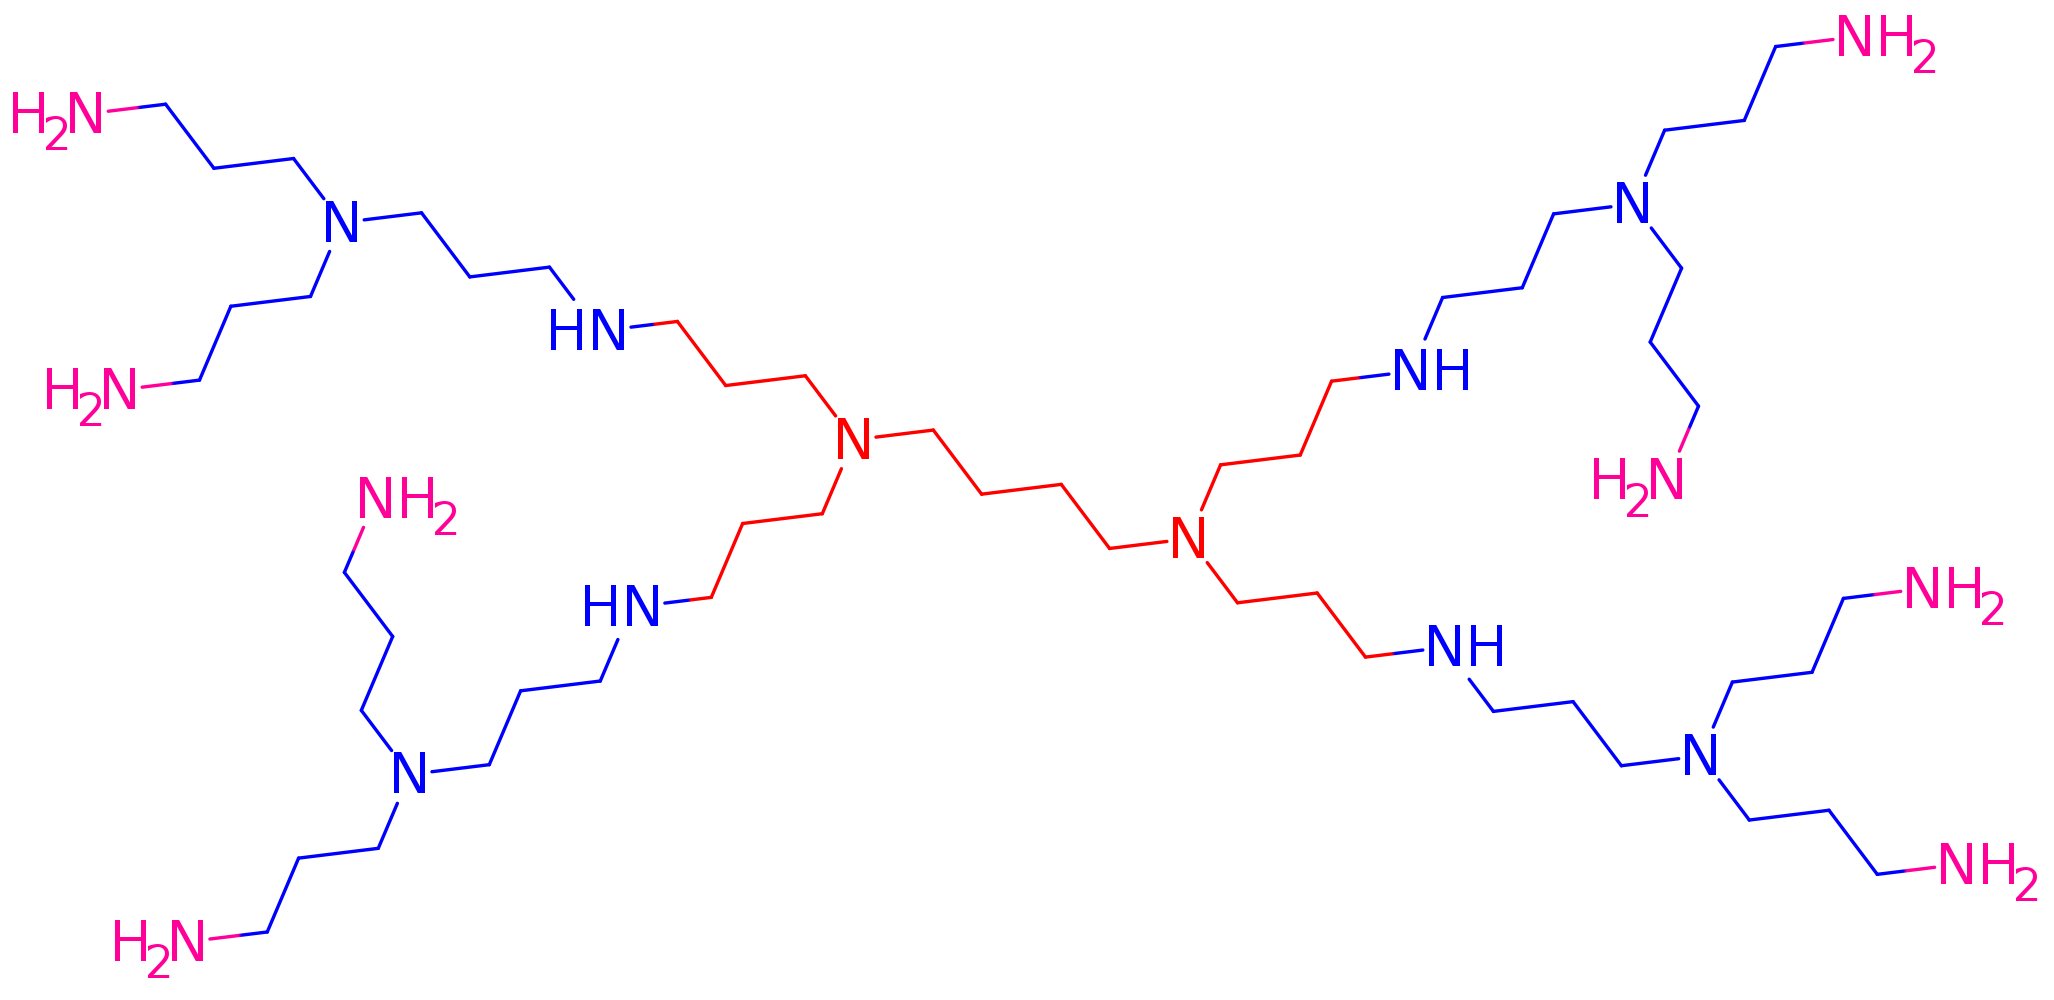
\includegraphics[width=0.5\textwidth]{PPI/PPIG1.png}
    \caption{PPI G1 dendrimer.
             The color code is adopted from Figure \ref{fig:PPIBB}.}
    \label{fig:PPIG1}
\end{figure}

It is worth noticing that protonated BBs were also provided.
The interested user is welcome to use them.
They have the same file name than the unprotonated BBs but with the suffix ``-protonated''.
Protonated BBs were omitted from the directory tree for simplicity.

After pyPolyBuilder finished the optimization step, any visualization software can be used to check the output geometry. 
Since the coordinates are generated considering the molecule in vaccum, its conformation may not be the expected solvated one (see Figure \ref{fig:PPIG1PPB}).
For that reason, the run directory has some scripts to run a short MD simulation in order to equilibrate the molecule in water using gromacs.
However, these scripts were developed for a specific architecture and need to be adapted by each user.

\begin{figure}
    \centering
    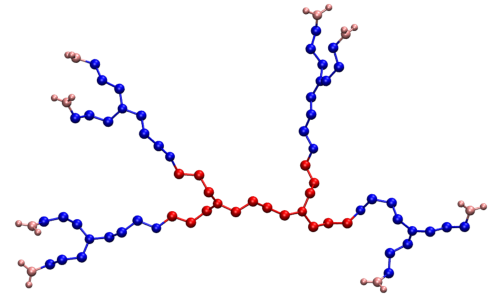
\includegraphics[width=0.5\textwidth]{PPI/PPI.pdf}
    \caption{PPI G1 dendrimer built by pyPolyBuilder.
             The color code is the same as in Figure \ref{fig:PPIBB}.}
    \label{fig:PPIG1PPB}
\end{figure}

PPI.sh is a script to automatically solvate, minimize energy, equilibrate for 100 ps using nvt and npt ensemble and run 100 ps of molecular dynamic simulation.
The simulation time is actually too small for simulating dendrimers. With this tutorial, we only intend to illustrate how pyPolyBuilder can be used in the creation of a molecular model.
PPI.top is the topology file for the system and mdp directory have all required mdp files.
However, these scripts were developed for a specific architecture and need to be adapted by each user.
For instance, the path for gromacs needs to be adapted and the output from pyPolyBuilder (PPI.gro and PPI.itp) needs to be moved to run directory.

After carrying out the solvation, energy minimization and 100 ps of both nvt and npt equilibrations, PPI dendrimer is in a more reasonable conformation (Figure \ref{fig:PPIG1SOL}).

\begin{figure}
    \centering
    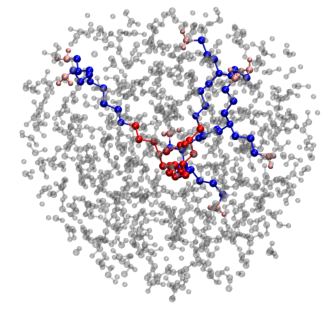
\includegraphics[width=0.5\textwidth]{PPI/PPISOL.pdf}
    \caption{PPI G1 dendrimer in water solution.
             The color code is the same as in Figure \ref{fig:PPIBB}.
             Water molecules are represented as translucent gray molecules.}
    \label{fig:PPIG1SOL}
\end{figure}